\documentclass[11pt]{article}


\usepackage[hmargin={0.6in, 0.6in}, vmargin={0.9in, 0.9in}]{geometry}
\usepackage{amsmath, amsthm, booktabs}
\usepackage{amssymb}
\usepackage{pdfpages}
\usepackage{setspace}
\usepackage{booktabs}
\usepackage{graphicx}
\usepackage{url} 
\usepackage{tikz}
\usetikzlibrary{automata, arrows}
\usepackage{pgfplots}
\pgfplotsset{compat=1.15}
\usepackage{mathrsfs}

\newcommand{\dif}{\mathrm{d}}
\newcommand{\Var}{\mathbb{V}}
\newcommand{\PP}{\mathbb{P}}
\newcommand{\EE}{\mathbb{E}}
\newcommand{\LL}{\mathbb{L}}


%\usepackage{fancyheadings}
%\usepackage{hyperref}

\renewcommand{\baselinestretch}{1}

\newtheorem{proposition}{Proposition}

\title{Likelihood of the model for the branching process}
\author{Author}
\date{October 2025}

\begin{document}

\maketitle

Supposed the process starts at time $T_0 = 0$ and the number of starting stem cell $S_0$. The interarrival time of the next event is exponentially distributed

$$\Delta_{T_i} = T_i - T_{i-1} \sim \text{Exp}(r\cdot S_{i-1}), \, i = 1, \cdots, n,$$

where $r$ is the division rate. At the event time $T_i$, the triplet of random variable $(X_i, Y_i, Z_i)$ has the following distribution
\begin{equation}
    (X_i, Y_i, Z_i) = \begin{cases}
        (+1, 0, 0), & p_1(T_i)\\
        (0, +1, 0), & p_2(T_i)\\
        (-1, +2, 0), &p_3(T_i) \\
        (0, 0, +1), & p_4(T_i).
    \end{cases}
\end{equation}
Assume that there is no dud stem cells (i.e $p_4(t) = 0 \, \forall t)$, and we observe all the events (both the time of the events $T_0, T_1, \cdots, T_n$, and the number of stem cells $S_0, S_1, \cdots, S_n$. Since we observe every events, we can know how the cell changes $(X_i, Y_i)$ at each event time.

The likelihood of observing the event times and division types \begin{equation}
    \LL(T_1, T_2, \cdots, T_n, S_1, \cdots, S_i) = \prod_{i=1}^n \Big[p_1(T_i) I_{(X_i=1)} + p_2(T_i) I_{(X_i=0)} + p_3(T_i) I_{(X_i=-1)}\Big] \cdot rS_{i-1}e^{-rS_{i-1} \Delta_{T_i}}.
\end{equation}
Given the division probability
\begin{equation}
\begin{split}
    P(X_i = 1 \vert T_i) & = \frac{p_1}{1 + c(T_i-m)^2} \\
    P(X_i = 0 \vert T_i) & = \frac{p_2}{1 + c(T_i-m)^2} \\
    P(X_i = -1 \vert T_i) & = 1-\frac{p_1 + p_2}{1 + c(T_i-m)^2},
\end{split}
\end{equation}
with $p_1, p_2, c, m > 0, p_1 + p_2 < 1$, the likelihood of observing the event is
\begin{equation}
\begin{split}
       &\LL(T_1, T_2, \cdots, T_n, S_1, \cdots, S_i) \\
       & = \prod_{i=1}^n \Big[ \frac{p_1}{1 + c(T_i-m)^2}I_{(X_i=1)} + \frac{p_2}{1 + c(T_i-m)^2} I_{(X_i=0)} + \Big( 1- \frac{p_1 + p_2}{1 + c(T_i-m)^2}\Big) I_{(X_i=-1)}\Big] rS_{i-1}e^{-rS_{i-1} \Delta_{T_i}}. 
\end{split}
\end{equation}
Let $f(t, c,m) = \frac{1}{1+c(t-m)^2}$, the log-likelihood is
\begin{equation}
    \begin{split}
        &\ell(T_1, T_2, \cdots, T_n, S_1, \cdots, S_n) \\
        &= \sum_{i=1}^n \Big[\log (p_1 \cdot  f(T_i, c,m)) \cdot I_{(X_i = 1)} +  \log (p_2 \cdot  f(T_i, c,m)) \cdot I_{(X_i = 0)} + \log ([ 1- (p_1+p_2)] \cdot  f(T_i, c,m)) \cdot I_{(X_i = -1)}\Big] \\
        & + n \log(r) + \sum_{i=1}^n \log (S_{i-1}) -r\sum_{i = 1}^n S_{i-1} \Delta_{T_i}.
    \end{split}
\end{equation}
We take derivative of the log-likelihood with respect to each parameter $r, p_1, p_2, c, m$
\begin{equation}
    \begin{split}
    \frac{\partial \ell}{\partial r} &= \frac{n}{r} - \sum_{i=1}^n S_{i-1} \Delta_{T_i},\\
    \frac{\partial \ell}{\partial p_1} &= \sum_{i=1}^n \frac{I_{(X_i = 1)}}{p_1} -\sum_{i=1}^n \frac{I_{(X_i = -1)} f(T_i, c,m)}{1-(p_1 + p_2) f(T_i, c, m)}, \\
    \frac{\partial \ell}{\partial p_2} &= \sum_{i=1}^n \frac{I_{(X_i = 0)}}{p_2} -\sum_{i=1}^n \frac{I_{(X_i = -1)} f(T_i, c,m)}{1-(p_1 + p_2) f(T_i, c, m)}, \\
    \frac{\partial \ell}{\partial c} & = \sum_{i=1}^n \frac{I_{(X_i = 1)} + I_{(X_i = 0)}}{f(T_i, c, m)} [-(T_i -m)^2 f(T_i, c,m)] \\
    & - \sum_{i=1}^n \frac{I_{(X_i = -1)} (p_1 + p_2)}{1-(p_1 + p_2 ) f(T_i, c, m)} [-(T_i -m)^2 f(T_i, c,m)], \\
    \frac{\partial \ell}{\partial m} & = \sum_{i=1}^n \frac{I_{(X_i = 1)} + I_{(X_i = 0)}}{f(T_i, c, m)} 2c(T_i-m)[f(T_i,c,m)]^2 \\
    &- \sum_{i=1}^n \frac{I_{(X_i = -1)} (p_1 + p_2)}{1-(p_1 + p_2 ) f(T_i, c, m)}2c(T_i-m)[f(T_i,c,m)]^2.
    \end{split}
\end{equation}
Setting $\frac{\partial \ell}{\partial r} = 0,$ we have 
$$\hat{r} = \frac{n}{\sum_{i=1}^n S_{i-1} \Delta_{T_i}}.$$
So we can get a closed-form solution for the MLE of parameter $r$.

\subsection*{MLE Estimates}
I use the log-likelihood function in equation (5) and optimize it using the Nelder-Mead optimization in R with linear inequality constraints (function constrOptim) to estimates the parameters. I also include the gradients from equation (6) in the optimization. I simulate 100 replications using the parameters $S_0 = 200, r = 0.2, p_1 = 0.5, p_2 = 0.2, c = 0.005, m = 4$. Figure (\ref{fig:prob_function}) shows the probability function given these parameters.

\begin{figure}[!ht]
    \centering
    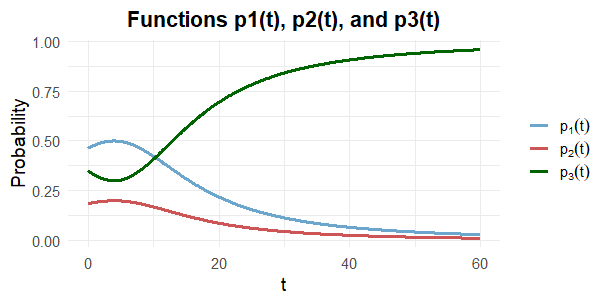
\includegraphics[width=0.75\linewidth]{prob_plot_05020005402.png}
    \caption{Functions $p_1(t), p_2(t), p_3(t)$ with parameters $p_1 = 0.5, p_2 = 0.2, c = 0.005, m = 4.$}
    \label{fig:prob_function}
\end{figure}
The estimates are stable at different starting points. Figure (\ref{fig:start01}) and table (\ref{tab:start01}) show estimates and their summary statistics across 100 replications with starting value $(p_1, p_2, c, m,r) = (0.1, 0.1, 5, 5, 1)$. Figure (\ref{fig:start02}) and table (\ref{tab:start02}) show estimates and their summary statistics across 100 replications with starting value $(p_1, p_2, c, m,r) = (0.2, 0.4, 10, 10, 1)$. Both starting values give really good estimates across all parameters.
\begin{figure}[!ht]
    \centering
    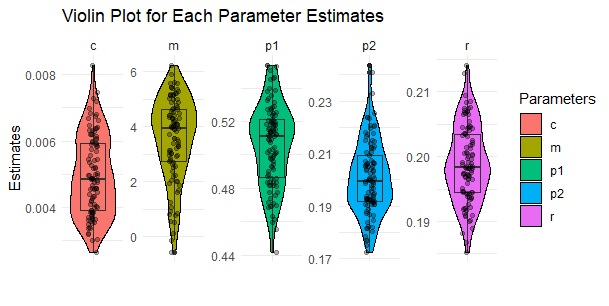
\includegraphics[width=0.75\linewidth]{start01_05020005402.png}
    \caption{Violin plot for estimate results using starting values $(p_1, p_2, c, m,r) = (0.1, 0.1, 5, 5, 1)$ with 100 replications. The true parameters are $(p_1, p_2, c, m,r) = (0.5, 0.2, 0.005, 4, 0.2)$.}
    \label{fig:start01}
\end{figure}
\begin{table}[!ht]
    \centering
    \begin{tabular}{|c|c|c|c|c|c|}
    \hline
         Parameter& $p_1$ & $p_2$ &$c$  & $m$ & $r$\\
         \hline
         Mean &  0.506 & 0.201 & 0.00495 & 3.550 & 0.199\\
         Median& 0.511 & 0.199 & 0.00485 & 3.940 & 0.198 \\
         2.5 Percentile& 0.461 & 0.177 & 0.00311 & 0.315 & 0.188 \\
         97.5 Percentile& 0.552 & 0.229 & 0.00723 & 5.590 & 0.209\\
         \hline
    \end{tabular}
    \caption{Parameter estimate results using starting values $(p_1, p_2, c, m,r) = (0.1, 0.1, 5, 5, 1)$ with 100 replications. The true parameters are $(p_1, p_2, c, m,r) = (0.5, 0.2, 0.005, 4, 0.2)$.}
    \label{tab:start01}
\end{table}

\begin{figure}[!ht]
    \centering
    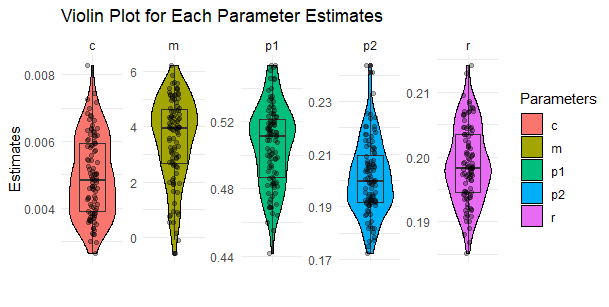
\includegraphics[width=0.75\linewidth]{start02_05020005402.png}
    \caption{Violin plot for estimate results using starting values $(p_1, p_2, c, m,r) = (0.2, 0.4, 10, 10, 1)$ with 100 replications. The true parameters are $(p_1, p_2, c, m,r) = (0.5, 0.2, 0.005, 4, 0.2)$.}
    \label{fig:start02}
\end{figure}
\begin{table}[!ht]
    \centering
    \begin{tabular}{|c|c|c|c|c|c|}
    \hline
         Parameter& $p_1$ & $p_2$ &$c$  & $m$ & $r$\\
         \hline
         Mean &  0.506 & 0.201 & 0.00495 & 3.530 & 0.199\\
         Median& 0.511 & 0.200 & 0.00482 & 3.960 & 0.198 \\
         2.5 Percentile& 0.462 & 0.177 & 0.00311 & 0.316 & 0.189 \\
         97.5 Percentile& 0.552 & 0.229 & 0.00723 & 5.590 & 0.209\\
         \hline
    \end{tabular}
    \caption{Parameter estimate results using starting values $(p_1, p_2, c, m,r) = (0.1, 0.1, 5, 5, 1)$ with 100 replications. The true parameters are $(p_1, p_2, c, m,r) = (0.5, 0.2, 0.005, 4, 0.2)$.}
    \label{tab:start02}
\end{table}

\subsection*{Simulation to include tracking of each cell time of division}
I'm also currently working on simulating data to track the time stem cells are created and undergo division. The simulation produces two datasets. The first one is the data that tracks cell counts after each division as we have before (figure (\ref{fig:division}). The second one is the data that tracks the parent cell of each cell and when each cell is created and ceased to exist (undergo division) (figure (\ref{fig:time}). Currently I have this tracking for viable stem cells only. I will add the tracking to the non-viable stem cells and differentiated cells as well. The goal is to used the information of the time cell is created to estimate whether it is a viable or non-viable stem cell.

\begin{figure}
    \centering
    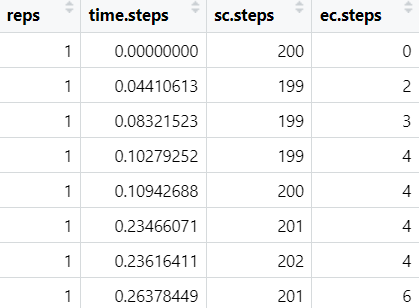
\includegraphics[width=0.5\linewidth]{trackingdivision.png}
    \caption{Simulated data that tracks the cell counts after each division.}
    \label{fig:division}
\end{figure}

\begin{figure}
    \centering
    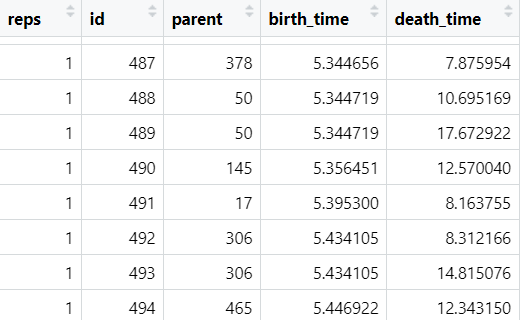
\includegraphics[width=0.5\linewidth]{trackingtime.png}
    \caption{Simulated data that tracks parent cells, birth time (when cell is created) and death time (when cell undergoes division and ceases to exists) of stem cell.}
    \label{fig:time}
\end{figure}
\newpage


\subsection*{Add $p_4$ to simplest form of probability function with $p_1, p_2, c, m$}
I tried to add $p_4$, probability of getting non-viable stem cells, to the simplest form of the probability function with parameters $p_1, p_2, c, m$
\begin{equation}
\begin{split}
    P((X_i, Z_i) = (1,0) \vert T_i) & = \frac{p_1}{1 + c(T_i-m)^2} \\
    P((X_i, Z_i) = (0,0) \vert T_i) & = \frac{p_2}{1 + c(T_i-m)^2} \\
    P((X_i, Z_i) = (-1,0) \vert T_i) & = 1-p_4 -\frac{p_1 + p_2}{1 + c(T_i-m)^2} \\
    P((X_i, Z_i) = (0,1)\vert T_i) & = p_4,
\end{split}
\end{equation}
When we observe viable and non-viable stem cells separately, the likelihood of observing the event times and division outcomes
\begin{equation}
    \begin{split}
        &\LL(T_1, T_2, \cdots, T_n, S_1, \cdots, S_i) \\= 
        & \prod_{i=1}^n \Big[p_1(T_i) I_{(X_i=1, Z_i = 0)} + p_2(T_i) I_{(X_i=0, Z_i = 0)} + p_3(T_i) I_{(X_i=-1, Z_i = 0)}+ p_4(T_i) I_{(X_i = 0, Z_i = 1)}\Big] rS_{i-1}e^{-rS_{i-1} \Delta_{T_i}}.
    \end{split}
\end{equation}
I simulate 100 replications using the parameters $S_0 = 200, r = 0.2, p_1 = 0.5, p_2 = 0.2, p_4 = 0.05, c = 0.005, m = 4$. Table (\ref{tab:simple_with_p4_start01}) and (\ref{tab:simple_with_p4_start02}) show the estimate results with two different starting values. The estimates are very stable and accurate. 

% \begin{figure}[!ht]
%     \centering
%     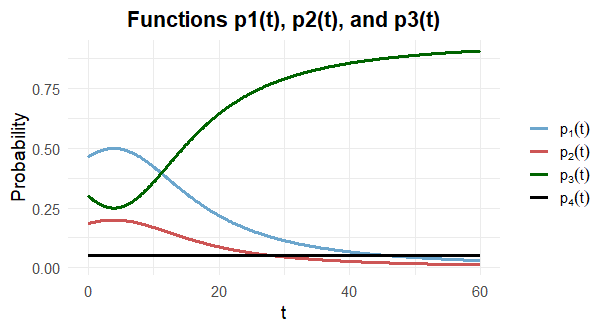
\includegraphics[width=0.75\linewidth]{prob_plot_05020005402005.png}
%     \caption{Functions $p_1(t), p_2(t), p_3(t), p_4(t)$ with parameters $p_1 = 0.5, p_2 = 0.2, p_4 = 0.05,  c= 0.005, m = 4$}
%     \label{fig:placeholder}
% \end{figure}

% \begin{figure}[!ht]
%     \centering
%     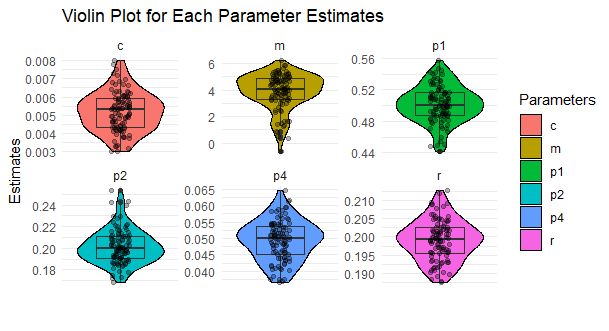
\includegraphics[width=0.75\linewidth]{start01_05020005402005.png}
%     \caption{start 01}
%     \label{fig:placeholder}
% \end{figure}

\begin{table}[!ht]
    \centering
    \begin{tabular}{|c|c|c|c|c|c|c|}
    \hline
         Parameter& $p_1$ & $p_2$ &$p_4$ &$c$  & $m$ & $r$\\
         \hline
         Mean &  0.502 & 0.202 & 0.049 & 0.00519 & 3.870 & 0.199\\
         Median& 0.500 & 0.200 & 0.050 & 0.00530 & 4.060 & 0.199  \\
         2.5 Percentile& 0.450 & 0.174 & 0.037 & 0.00321 & 0.641 & 0.189 \\
         97.5 Percentile& 0.544 & 0.241 & 0.060 & 0.00741 & 5.730 & 0.209\\
         \hline
    \end{tabular}
    \caption{Parameter estimate results for the simplest form of the probability function with non-viable stem cells. The true parameters are $(p_1, p_2, p_4, c, m) = (0.5, 0.2, 0.05, 0.005, 4)$. The starting values are $(p_1, p_2, p_4, c, m) = (0.1, 0.1, 0.1, 5, 5, 1)$.}
    \label{tab:simple_with_p4_start01}
\end{table}

% \begin{figure}[!ht]
%     \centering
%     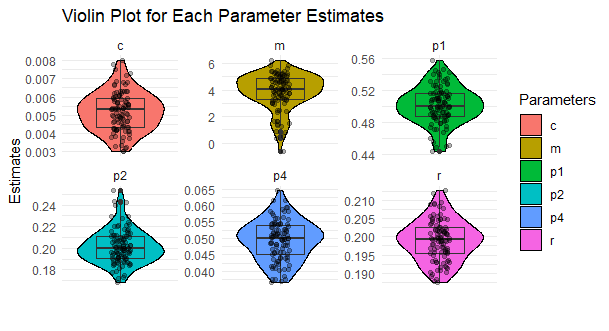
\includegraphics[width=0.75\linewidth]{start02_0502000540205.png}
%     \caption{start02}
%     \label{fig:placeholder}
% \end{figure}

\begin{table}[!ht]
    \centering
    \begin{tabular}{|c|c|c|c|c|c|c|}
    \hline
         Parameter& $p_1$ & $p_2$ &$p_4$ &$c$  & $m$ & $r$\\
         \hline
         Mean &  0.502 & 0.202 & 0.049 & 0.00519 & 3.880 & 0.199\\
         Median& 0.500 & 0.200 & 0.050 & 0.00529 & 4.080 & 0.199  \\
         2.5 Percentile& 0.450 & 0.174 & 0.037 & 0.00320 & 0.641 & 0.189 \\
         97.5 Percentile& 0.544 & 0.241 & 0.060 & 0.00741 & 5.730 & 0.209\\
         \hline
    \end{tabular}
    \caption{Parameter estimate results for the simplest form of the probability function with non-viable stem cells. The true parameters are $(p_1, p_2, p_4, c, m) = (0.5, 0.2, 0.05, 0.005, 4)$. The starting values are $(p_1, p_2, p_4, c, m) = (0.2, 0.4, 0.1, 20, 20, 1)$.}
    \label{tab:simple_with_p4_start02}
\end{table}
\newpage
\clearpage
\subsection*{Variance of Cell Count in Branching Process}
\subsubsection*{Derivation of the theoretical expectation and variance}
Let $\Delta > 0$. 
\begin{equation}
    \begin{split}
        E[X(t + \Delta) - X(t) \vert X(t)] & = [p_1(t) - p_3(t) + \mathcal{O}(\Delta)] \cdot r X(t) \Delta + \mathcal{o}(\Delta) \\
        & = [p_1(t) - p_3(t)] rX(t) + \mathcal{o}(\Delta).
    \end{split}
\end{equation}
Taking expectation,
\begin{equation}
    \begin{split}
        S(t + \Delta) - S(t) = [p_1(t) - p_3(t)] r S(t) \Delta + E[\xi] + \mathcal{o}(\Delta).
    \end{split}
\end{equation}
Let $\Delta \rightarrow 0$,
\begin{equation}
    \frac{dS(t)}{dt} = [p_1(t) - p_3(t)]rS(t).
\end{equation}
Thus, the expected stem cell count of the branching process coincides with the differential equation.

Let $V(t)$ denote the theoretical variance of the stem cell in the branching process. Denote $S(t) = E[X(t)], M(t) = E[X(t)^2]$, then $V(t) = M(t) - S(t)^2$. Let $\Delta > 0$.
\begin{equation}
    \begin{split}
        E[X(t + \Delta)^2 - X(t)^2 \vert X(t)] & = [2 X(t) (p_1(t) - p_3(t)) + (p_1(t) + p_3(t))] rX(t) \Delta\\
        & = 2 X(t)^2(p_1(t)-p_3(t)) r \Delta + X(t) (p_1(t) + p_3(t) ) r\Delta.
    \end{split}
\end{equation}
Taking expectation,
\begin{equation}
    \begin{split}
        M(t + \Delta) - M(t) = 2[p_1(t) -p_3(t)] rM(t) \Delta + [p_1(t) + p_3(t)] rS(t) \Delta.
    \end{split}
\end{equation}
Let $\Delta \rightarrow0$,
\begin{equation}
\begin{split}
    M'(t) &= 2[p_1(t) -p_3(t)]rM(t) + [p_1(t) + p_3(t)]rS(t),\\
    V'(t) & = M'(t)  - 2S(t) S'(t) \\
    & = 2[p_1(t) - p_3(t)] rM(t) + [p_1(t) + p_3(t)]rS(t) - 2S(t)[p_1(t) - p_3(t)]rS(t) \\
    & = 2[p_1(t) -p_3(t)]rV(t) + [p_1(t) + p_3(t)]r S(t).
\end{split}
\end{equation}
\subsubsection*{Verify the theoretical variance with simulation}
Figure (\ref{fig:var_compare}) displays the plots to compare variance from the branching process with variance from the compound nonhomogeneous Poisson process, using the form of the probability function 
\begin{equation}
    \begin{split}
        P(X_i = 1 \vert T_i) &= \frac{p_1}{1 + c_1 (T_i -m_1)^2}, \\
        P(X_i = 0 \vert T_i) & = \frac{p_2}{1 + c_2 (T_i - m_2)^2}, \\
        P(X_i = -1 \vert T_i ) & = 1- \frac{p_1}{1+c_1(T_i -m_1)^2} - \frac{p_2}{1 + c_2(T_i -m_2)^2}.
    \end{split}
\end{equation}
The parameters used to construct these plots are $S_0 = 200, r = 0.2, p_1 = 0.5, c_1 = 0.005, m_1 = 4, p_2 = 0.2, c_2 = 0.1, m_2 = 12$. Figure (\ref{fig:var_compare}) on the left is the plot of variances over time, and on right is the theoretical mean and the region within two standard deviations from the mean. In this set-up, the theoretical variances of the two processes start out similar in the beginning, however, as $t$ gets large, the variance of the branching process converges to 0, whereas the variance of the compound nonhomogeneous Poisson process converges to a positive number. It is also possible for the variance of the branching process to be greater than that of the compound Poisson process. 

\begin{figure}[!h]
    \centering
    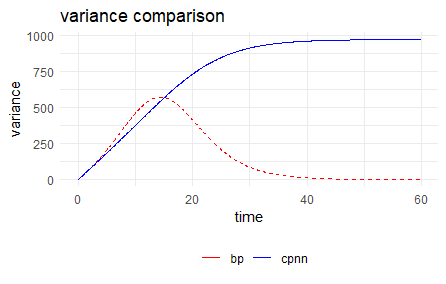
\includegraphics[width=0.45\linewidth]{variance_comparison.png}
    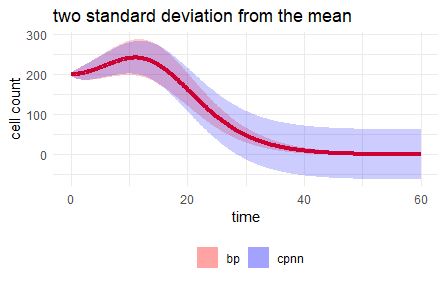
\includegraphics[width=0.45\linewidth]{sdfrommean.png}
    \caption{Comparing theoretical variances of the two process with parameters $S_0 = 200, r = 0.2, p_1 = 0.5, c_1 = 0.005, m_1 = 4, p_2 = 0.2, c_2 = 0.1, m_2 = 12$}
    \label{fig:var_compare}
\end{figure}
Figure (\ref{fig:var_sim}) compares the theoretical variances with the variability from the simulated data. 50 replications of the simulated data with the same parameters as in figure (\ref{fig:var_compare}). The simulated cell count data is plotted, along with the theoretical mean and the region within 2 theoretical standard deviation from the mean. 

\begin{figure}[!ht]
    \centering
    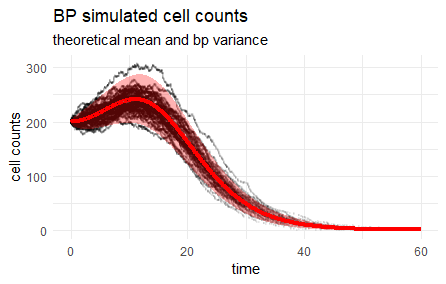
\includegraphics[width=0.45\linewidth]{bpCI.png}
    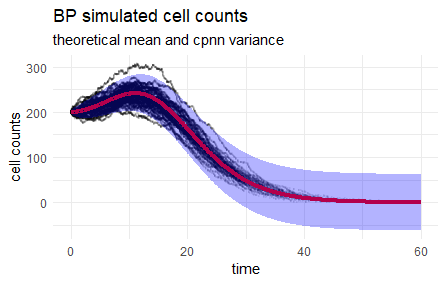
\includegraphics[width=0.45\linewidth]{cpnnCI.png}
    \caption{Compare theoretical variances with the simulated data with parameters $S_0 = 200, r = 0.2, p_1 = 0.5, c_1 = 0.005, m_1 = 4, p_2 = 0.2, c_2 = 0.1, m_2 = 12$.}
    \label{fig:var_sim}
\end{figure}
\subsubsection*{Show variance of the stem cell is finite }
$$V'(t) = 2[p_1(t) - p_3(t)] r V(t) + [p_1(t) + p_3(t)]r S(t),$$
\begin{equation}
    \begin{split}
        \Rightarrow V(t) &= \exp \Big\{ 2r\int_0^t [p_1(u) -p_3(u)] du  \Big\} \Big[\int_0^t [p_1(u) + p_3(u)] r S(u)  \exp \Big\{ -2r\int_0^u [p_1(v) -p_3(v)] dv  \Big\}du + C \Big] \\
        & = \exp \Big\{ 2r\int_0^t [p_1(u) -p_3(u)] du  \Big\} \\
        & \quad
        \Big[\int_0^t [p_1(u) + p_3(u)] r S_0 \exp \Big\{ r\int_0^u [p_1(v) -p_3(v)] dv  \Big\} \exp \Big\{ -2r\int_0^u [p_1(v) -p_3(v)] dv  \Big\}du + C \Big] \\
        & = S_0 \cdot r \cdot \exp \Big\{ 2r\int_0^t [p_1(u) -p_3(u)] du  \Big\} \Big[\int_0^t [p_1(u) + p_3(u)] 
        \exp \Big\{ -r\int_0^u [p_1(v) -p_3(v)] dv  \Big\}du + C \Big].
    \end{split}
\end{equation}
Using the initial condition $V(0) = 0$, we can simplify the expression of $V(t)$ in terms of $S(t)$

$$V(t) = r S(t)^2 \int_0^t \frac{p_1(u) + p_3(u)}{S(u)} du.$$

Let $P(t) = \int_0^t [p_1(u) -p_3(u)] du$. Since $p_1(u) + p_3(u) \leq 1 \ \forall u$ and $r$ is a positive constant, to show $V(t) < \infty$ as $t \rightarrow \infty$, we can show 
$$f (t) = \exp \Big\{ P(t) \Big\} \Big[\int_0^t\exp \Big\{ - P(u)  \Big\}du \Big] < \infty $$ as $t \rightarrow \infty$. 
When $P(t) \rightarrow \infty$, $\exp \Big\{  P(t) \Big\} \rightarrow \infty$ and $\int_0^t\exp \Big\{ - P(u)  \Big\}du < \infty$ as $t \rightarrow \infty$. Then $f(t) \rightarrow \infty$ as $t\rightarrow \infty$. Thus, we consider when $P(t) \rightarrow - \infty$ as $t \rightarrow \infty$.

We rewrite $f(t)$ as a quotient
$$f(t) = \frac{\int_0^t\exp \Big\{ - P(u)  \Big\}du }{\exp \Big\{ - P(t) \Big\}}.$$
Both numerator and denominator go to $+ \infty$ as $t \rightarrow \infty$, we can use the l'H\^opital's rule.
$$\lim_{t\rightarrow \infty} f(t) = \lim_{t\rightarrow \infty} \frac{\int_0^t\exp \Big\{ - P(u)  \Big\}du}{\exp \Big\{ - P(t) \Big\}} = \lim_{t\rightarrow \infty} = \frac{\exp \{ - P(t) \}} {-[p_1(t) - p_3(t)] \exp \{ - P(t) \}} =  \lim_{t\rightarrow \infty} \frac{-1}{p_1(t) - p_3(t)}.$$

\textbf{Case 1.} $\lim_{t\rightarrow \infty} [p_1(t) - p_3(t)] \rightarrow - p$ for some $p > 0$. Then $\lim_{t\rightarrow \infty} f(t)$ is a finite constant.

\textbf{Case 2.} $\lim_{t\rightarrow \infty} [p_1(t) - p_3(t)] \rightarrow - \infty$. Then $\lim_{t\rightarrow \infty} f(t) \rightarrow 0$.

\textbf{Case 3.} $[p_1(t) - p_3(t)]$ does not converge but is negative on average $$\limsup_{T\rightarrow\infty} {\frac{1}{T} \int_0^T [p_1(u) - p_3(u)] du = \limsup_{T\rightarrow\infty} \frac{P(T)}{T} = \bar{p}} < 0.$$
Then on average $P(t)$ decreases roughly like $\bar{p}t$ for large $t$ with some remainder term $P(t) = \bar{p}t + R(t)$, that is bounded or growing slower than linear. Then
\begin{equation}
    \begin{split}
        f (t) &= \exp \Big\{ P(t) \Big\} \Big[\int_0^t\exp \Big\{ - P(u)  \Big\}du\Big] \\
        & = \exp \{\bar{p}t + R(t)\} \int_0^t \exp \{-\bar{p}u - R(u)\} du \\
        & = \exp \{\bar{p}t\} \exp\{R(t)\} \int_0^t \exp \{\vert\bar{p} \vert u\} \exp \{-R(u)\} du \ (\text{since } \bar{p} < 0). 
    \end{split}
\end{equation}
Since $R(t)$ oscillates and is bounded, $\exp\{-R(u)\}$ is bounded. Thus, $\int_0^t \exp \{\vert\bar{p} \vert u\} \exp \{-R(u)\} du  \approx C_1 \exp \{\vert\bar{p} \vert t\} $ for some $C > 0$. Then
$$f(t) \approx \exp \{\bar{p}t\} \exp\{R(t)\} C_1 \exp \{\vert\bar{p} \vert t\} = C_1 \exp\{R(t)\}.$$
Since $\exp\{R(u)\}$ is bounded, $f(t)$ is bounded. Thus, as $t \rightarrow \infty$ the variance $V(t)$ is finite when $\int_0^t [p_1(u) - p_3(u)]du \rightarrow -\infty$. $V(t) \rightarrow 0$ when $[p_1(t) - p_3(t)] \rightarrow -\infty$. 
\newpage

\subsection*{Add parameters for $p_2(t)$}
Suppose we have the division probabilities
\begin{equation}
    \begin{split}
        P(X_i = 1 \vert T_i) & = \frac{p_1}{1+c_1(T_i-m_1)^2},\\
        P(X_i = 0 \vert T_i) & = \frac{p_2}{1+c_2(T_i-m_2)^2},\\
        P(X_i = -1 \vert T_i) & = 1-\frac{p_1}{1+c_1(T_i-m_1)^2} - \frac{p_2}{1+c_2(T_i-m_2)^2},
    \end{split}
\end{equation}
with $p_1, p_2, c, m > 0, p_1 + p2 < 1$. The likelihood of observing the event is 
\begin{equation}
    \begin{split}
        \LL (T_1, \cdots, T_n, S_0, \cdots, S_n) 
        = \prod_{i=1}^n \Big[& \frac{p_1}{1+c_1(T_i-m_1)^2} I_{(X_i = 1)} + \frac{p_2}{1+c_2(T_i-m_2)^2} I_{(X_i = 0)} \\
        &+ \Big( 1- \frac{p_1}{1+c_1(T_i-m_1)^2} - \frac{p_2}{1+c_2(T_i-m_2)^2} I_{(X_i = -1)} \Big) \Big] rS_{i-1} e^{-rS_{i-1} \Delta_{T_i}}.
    \end{split}
\end{equation}
The log-likelihood is
\begin{equation}
    \begin{split}
        \ell(T_1, \cdots, T_n, S_0, \cdots, S_n) = \sum_{i=1}^n \Big[ &\log \Big(\frac{p_1}{1+c_1(T_i-m_1)^2}\Big) I_{(X_i = 1)} \\
        & + \log \Big(\frac{p_2}{1+c_2(T_i-m_2)^2}\Big) I_{(X_i = 0)} \\
        & + \log \Big(1- \frac{p_1}{1+c_1(T_i-m_1)^2}- \frac{p_2}{1+c_2(T_i-m_2)^2} \Big) I_{(X_i = -1)} \\
        & + \log r + \log S_{i-1} - rS_{i-1}\Delta_{T_1} \Big].
    \end{split}
\end{equation}
We take the derivative of the log-likelihood with respect to each parameter $r, p_1, p_2, c_1, c_2, m_1, m_2$.
\begin{equation}
    \begin{split}
        \frac{\partial \ell}{\partial r} & = \frac{n}{r} - \sum_{i=1}^nS_{i-1} \Delta_{T_I} \\
        \frac{\partial \ell}{\partial p_1} & = \sum_{i=1}^n \frac{I_{(X_i = 1)}}{p_1} - \sum_{i=1}^n \frac{I_{(X_i = -1)}}{1-\frac{p_1}{1+c_1(T_i-m_1)^2} - \frac{p_2}{1+c_2(T_i-m_2)^2}}\frac{1}{1+c_1(T_i-m_1)^2}\\
        \frac{\partial \ell}{\partial p_2} & = \sum_{i=1}^n \frac{I_{(X_i = 0)}}{p_2} - \sum_{i=1}^n \frac{I_{(X_i = -1)}}{1-\frac{p_1}{1+c_1(T_i-m_1)^2} - \frac{p_2}{1+c_2(T_i-m_2)^2}}\frac{1}{1+c_1(T_i-m_1)^2}\\
        \frac{\partial \ell}{\partial c_1} & = - \sum_{i=1}^n \frac{I_{(X_i = 1)} (T_i -m_1)^2}{1+c_1(T_i-m_1)^2}- \sum_{i=1}^n \frac{I_{(X_i = -1)}}{1-\frac{p_1}{1+c_1(T_i-m_1)^2} - \frac{p_2}{1+c_2(T_i-m_2)^2}} \Big( - \frac{p_1(T_i-m_1)^2}{[1+c_1(T_i-m_1)^2]^2}\Big)\\
        \frac{\partial \ell}{\partial c_2} & = - \sum_{i=1}^n \frac{I_{(X_i = 0)} (T_i -m_2)^2}{1+c_2(T_i-m_2)^2} - \sum_{i=1}^n \frac{I_{(X_i = -1)}}{1-\frac{p_1}{1+c_1(T_i-m_1)^2} - \frac{p_2}{1+c_2(T_i-m_2)^2}}\Big( - \frac{p_2(T_i-m_2)^2}{[1+c_2(T_i-m_2)^2]^2}\Big) \\
        \frac{\partial \ell}{\partial m_1} & = \sum_{i=1}^n \frac{I_{(X_i = 1)} 2c_1 (T_i -m_1)}{1+c_1(T_i-m_1)^2}- \sum_{i=1}^n \frac{I_{(X_i = -1)}}{1-\frac{p_1}{1+c_1(T_i-m_1)^2} - \frac{p_2}{1+c_2(T_i-m_2)^2}} \frac{2p_1 c_1(T_i-m_1)}{[1+ c_1(T_1-m_1)^2]^2}\\
        \frac{\partial \ell}{\partial m_2} & = \sum_{i=1}^n \frac{I_{(X_i = 0)} 2c_2(T_i -m_2)}{1+c_2(T_i-m_2)^2}- \sum_{i=1}^n \frac{I_{(X_i = -1)}}{1-\frac{p_1}{1+c_1(T_i-m_1)^2} - \frac{p_2}{1+c_2(T_i-m_2)^2}}\frac{2p_2 c_2(T_i-m_2)}{[1+ c_2(T_i-m_2)^2]^2}
    \end{split}
\end{equation}

% I simulate 100 replications using the parameters $S_0 = 200, r = 0.2, p_1 = 0.5, p_2 = 0.2, c_1 = 0.005, c_2 = 0.01, m_1 = 4, m_2 = 12$. Figure (\ref{fig:diffc_diffm}) shows the graphs of the probability function with these parameters. 

% \begin{figure}[!ht]
%     \centering
%     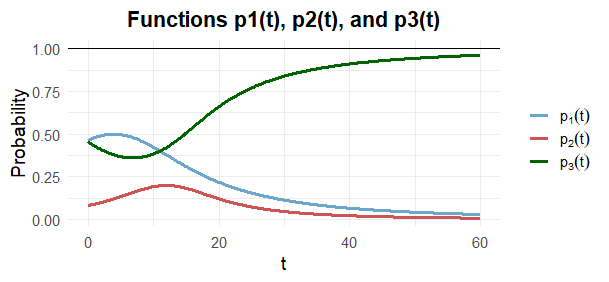
\includegraphics[width=0.75\linewidth]{prob_plot_diffc_diffm.png}
%     \caption{Function $p_1(t) = \frac{p_1}{1+ c_1(t-m_1)^2},p_2(t) = \frac{p_2}{1+ c_2(t-m_2)^2}, p_3(t) = 1- p_1(t)-p_2(t)$ with parameters $(p_1, p_2, c_1 ,c_2, m_1,m_2) = (0.5, 0.2, 0.005, 0.01, 4, 12)$}
%     \label{fig:diffc_diffm}
% \end{figure}

% I use the similar R function to optimize the log-likelihood function as before. The estimates were not good so I used the closed form solution of $\hat{r}$ to estimate the division rate $r$ and used the \textit{constrOptim} to optimize the condition likelihood given the time sequences $T_i's$ to obtain the parameters $p_1, p_2, c_1, c_2, m_1, m_2$. The estimates of $p_1$ and $p_2$ are pretty stable and pretty close to the true parameters. However, the estimates of other parameters, especially $m_1$ and $m_2$, are dependent of the starting values. Table (\ref{tab:diffc_diffm_start01}) and (\ref{tab:diffc_diffm_start02}) with two different starting values. The starting values used to obtained the estimates in (\ref{tab:diffc_diffm_start02}) have closer $m_1$ and $m_2$ to their true parameter values. 

% \begin{table}[!ht]
%     \centering
%     \begin{tabular}{|c|c|c|c|c|c|c|c|}
%     \hline
%          Parameter& $p_1$ & $p_2$ &$c_1$ &$c_2$ & $m_1$ & $m_2$ & $r^*$\\
%          \hline
%          Mean &  0.494 & 0.166 & 0.00438 & 0.00120 & 2.490 & 1.222 & 0.199\\
%          Median& 0.495 & 0.164 & 0.00365 & 0.00110 & 1.500 & 1.080 & 0.200  \\
%          2.5 Percentile& 0.442 & 0.140 & 0.00219 & 0.000473 & 0.0134 & 0.00110 & 0.189 \\
%          97.5 Percentile& 0.555 & 0.195 & 0.00706 & 0.00266 & 7.370 & 3.310 & 0.209\\
%          \hline
%     \end{tabular}
%     \caption{Parameters estimate results using starting values $(p_1, p_2, c_1 ,c_2, m_1,m_2) = (0.1, 0.1, 0.1, 0.1, 1, 1)$ with 100 replications. The true parameters are $(p_1, p_2, c_1 ,c_2, m_1,m_2) = (0.5, 0.2, 0.005, 0.01, 4, 12)$. *Estimates of $r$ is obtained from the closed form solution. }
%     \label{tab:diffc_diffm_start01}
% \end{table}



% \begin{table}[!ht]
%     \centering
%     \begin{tabular}{|c|c|c|c|c|c|c|c|}
%     \hline
%          Parameter& $p_1$ & $p_2$ &$c_1$ &$c_2$ & $m_1$ & $m_2$ & $r^*$\\
%          \hline
%          Mean &  0.501 & 0.187 & 0.00346 & 0.00698 & 1.38 & 9.440 & 0.199\\
%          Median& 0.500 & 0.186 & 0.00339 & 0.00583 & 1.250 & 9.470 & 0.200  \\
%          2.5 Percentile& 0.453 & 0.149 & 0.00210 & 0.00127 & 0.00149 & 4.610 & 0.189 \\
%          97.5 Percentile& 0.563 & 0.241 & 0.00532 & 0.0193 & 3.910  & 14.200 & 0.209\\
%          \hline
%     \end{tabular}
%     \caption{Parameters estimate results using starting values $(p_1, p_2, c_1 ,c_2, m_1,m_2) = (0.2, 0.7, 0.2, 0.2, 3, 10)$ with 100 replications. The true parameters are $(p_1, p_2, c_1 ,c_2, m_1,m_2) = (0.5, 0.2, 0.005, 0.01, 4, 12)$. *Estimates of $r$ is obtained from the closed-form solution. }
%     \label{tab:diffc_diffm_start02}
% \end{table}

% Instead of having different $c_1$ and $c_2$, I also tried having just one scale parameter $c$. The estimates are shown in table (\ref{tab:samec_diffm_start01}) (\ref{tab:samec_diffm_start02}). Similarly to when we have different $c_1$ and $c_2$, the estimates of $p_1$ and $p_2$ are stable, but estimates of $m_1$ and $m_2$ are not good.

% \begin{table}[!ht]
%     \centering
%     \begin{tabular}{|c|c|c|c|c|c|c|}
%     \hline
%          Parameter& $p_1$ & $p_2$ &$c$ & $m_1$ & $m_2$ & $r^*$\\
%          \hline
%          Mean &  0.450 & 0.223  & 0.00280  & 3.950 & 1.260     & 0.199\\
%          Median&  0.443 & 0.223  & 0.00256 & 3.820 & 0.368 & 0.198  \\
%          2.5 Percentile& 0.386 & 0.199  & 0.00173 & 0.0430 &0.00016 & 0.189 \\
%          97.5 Percentile& 0.498 & 0.251 & 0.00448 & 8.870 & 4.440 & 0.211\\
%          \hline
%     \end{tabular}
%     \caption{Parameters estimate results with same $c$ but different $m_1$ and $m_2$ using starting values $(p_1, p_2, c, m_1,m_2) = (0.1, 0.1, 0.1, 1, 1)$ with 100 replications. The true parameters are $(p_1, p_2, c_1 ,c_2, m_1,m_2) = (0.5, 0.2, 0.005, 4, 12)$. *Estimates of $r$ is obtained from the closed-form solution.}
%     \label{tab:samec_diffm_start01}
% \end{table}

% \begin{table}[!ht]
%     \centering
%     \begin{tabular}{|c|c|c|c|c|c|c|}
%     \hline
%          Parameter& $p_1$ & $p_2$ &$c$ & $m_1$ & $m_2$ & $r^*$\\
%          \hline
%          Mean &  0.504 & 0.195 & 0.00317 & 0.986 & 8.610 & 0.199\\
%          Median& 0.507 & 0.193 & 0.00319 & 0.374 & 8.930 & 0.198  \\
%          2.5 Percentile& 0.443 & 0.171 & 0.00236 & 0.00485 & 3.960 & 0.189 \\
%          97.5 Percentile& 0.552 & 0.229 & 0.00416 & 4.470 & 13.400 & 0.211\\
%          \hline
%     \end{tabular}
%     \caption{Parameters estimate results with same $c$ but different $m_1$ and $m_2$ using starting values $(p_1, p_2, c, m_1,m_2) = (0.2, 0.7, 0.2, 3, 10)$ with 100 replications. The true parameters are $(p_1, p_2, c_1 ,c_2, m_1,m_2) = (0.5, 0.2, 0.005, 4, 12)$. *Estimates of $r$ is obtained from the closed-form solution.}
%     \label{tab:samec_diffm_start02}
% \end{table}
I reviewed the code for the optimization of the log-likelihood function when we have the probability function as in (12) with different scale and location parameters ($c_1, c_2, m_1, m_2$) for $p_1(t)$ and $p_2(t)$. From the optimization results, the estimates for $p_1$ and $p_2$ are very stable, however, the estimates for $c_1, c_2, m_1, m_2$ are not. I ran the optimization multiple times with different starting points and chose the results with the highest log-likelihood. The starting points are shown in table (\ref{tab:starting_points}). Since $p_1$ and $p_2$ are not sensitive to starting values, the starting values for these two parameters are the same, whereas starting values for $c_1, c_2, m_1, m_2$ describe different scenarios of where the peaks and how sharp the peaks are in functions $p_1(t)$ and $p_2(t)$.
\begin{table}[!ht]
    \centering
    \begin{tabular}{|c|c|c|c|c|c|c|}
    \hline
         Scenarios & $p_1$ & $p_2$ &$c_1$ &$c_2$ & $m_1$ & $m_2$ \\
         \hline
         Early peaks&	0.3&	0.3&	0.05&	0.05&	10&	10\\
         Very early peaks&	0.3&	0.3&	0.05&	0.05&	5&	5\\
         Late peaks&	0.3&	0.3&	0.05&	0.05&	45&	45\\
         Sharp peak at center&	0.3&	0.3&	0.2&	0.2&	25&	25\\
         Broad peak at center&	0.3&	0.3&	0.001&	0.001&	25&	25\\
         Asymmetric time centers&	0.3&	0.3&	0.02&	0.03&	35&	15\\
         Asymmetric time centers&	0.3&	0.3&	0.1&	0.05&	20&	30\\
         Random start & unif(0.2,0.5) & unif(0.2,0.5) & unif(0.001,0.05) & unif(0.001,0.05) & unif(0,50) & unif(0,50)\\
         \hline
    \end{tabular}
    \caption{Multiple starting points for optimizations}
    \label{tab:starting_points}
\end{table}

Table (\ref{tab:multiple_start_case1}) and (\ref{tab:multiple_start_case2}) shows the estimate results for simulated data of two sets of parameters using the same multiple starting values. Both results are good and converge to the true parameters. I will try different optimization techniques to see if it would be less sensitive to starting points.

\begin{table}[!ht]
    \centering
    \begin{tabular}{|c|c|c|c|c|c|c|}
    \hline
         Parameter& $p_1$ (0.55)& $p_2$ (0.15) &$c_1$ (0.005) &$c_2$ (0.01) & $m_1$ (4)& $m_2$ (18) \\
         \hline
         Mean & 0.560 & 0.152& 0.00491 & 0.01120	& 3.340 & 17.600 \\
         Median	& 0.560 & 0.152 & 0.00479 & 0.01110 &3.820& 17.600 \\
         2.5 Percentile&	0.503&	0.107&	0.00292& 0.00374 &	0.0000416 & 14.200 \\
         97.5 Percentile &	0.621&	0.192&	0.00759&	0.02150&	6.570&	20.000\\
         \hline
    \end{tabular}
    \caption{Parameters estimate results using multiple starting values with 100 replications. The true parameters are $(p_1, p_2, c_1 ,c_2, m_1,m_2) = (0.55, 0.15, 0.005, 0.01, 4, 18)$.}
    \label{tab:multiple_start_case1}
\end{table}

\begin{table}[!ht]
    \centering
    \begin{tabular}{|c|c|c|c|c|c|c|}
    \hline
         Parameter& $p_1$ (0.2) & $p_2$ (0.7) &$c_1$ (0.005) &$c_2$ (0.01) & $m_1$ (12) & $m_2$ (6) \\
         \hline
         Mean&	0.200&	0.699&	0.00504&	0.01030&	10.700&	6.090\\
         Median&	0.197&	0.697&	0.00454&	0.01020&	10.400&	6.190\\
         2.5 Percentile&	0.163&	0.639&	0.00115&	0.00679&	5.590&	4.540\\
         97.5 Percentile&	0.244&	0.761&	0.01110&	0.01490&	14.800&	7.130\\
         \hline
    \end{tabular}
    \caption{Parameters estimate results using multiple starting values with 100 replications. The true parameters are $(p_1, p_2, c_1 ,c_2, m_1,m_2) = (0.2, 0.6, 0.005,0.1, 12, 6)$.}
    \label{tab:multiple_start_case2}
\end{table}

\newpage

\subsection*{Stopping times}

\begin{figure}[!ht]
    \centering
    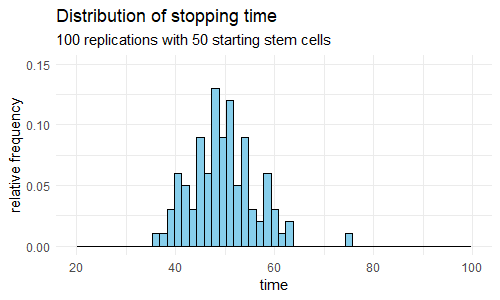
\includegraphics[width=0.45\linewidth]{stoppingtime_start50_rep100.png}
    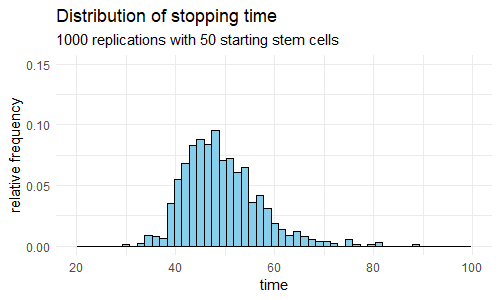
\includegraphics[width=0.45\linewidth]{stoppingtime_start50_rep1000.png}
    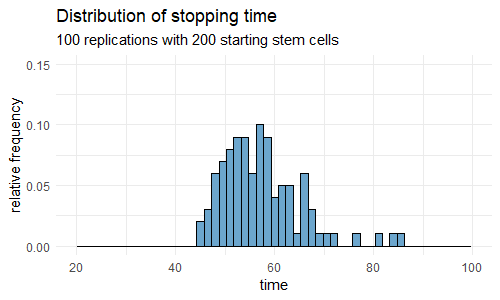
\includegraphics[width=0.45\linewidth]{stoppingtime_start200_rep100.png}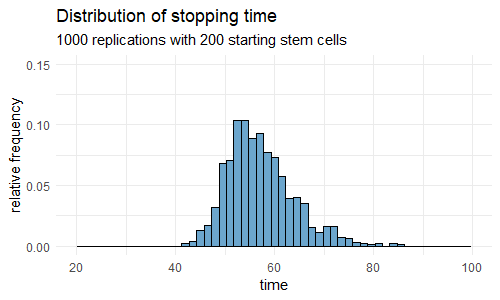
\includegraphics[width=0.45\linewidth]{stoppingtime_start200_rep1000.png}
    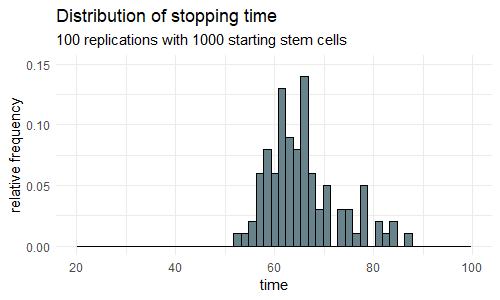
\includegraphics[width=0.45\linewidth]{stoppingtime_start1000_rep100.png}
    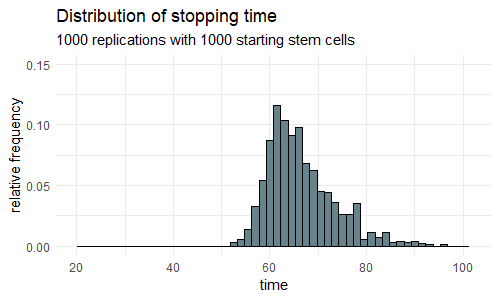
\includegraphics[width=0.45\linewidth]{stoppingtime_start1000_rep1000.png}
    \caption{Distributions of stopping times from simulated data with varying numbers of initial stem cells and replication counts. The number of starting stem cells is 50 (top row), 200 (middle row), and 1000 (bottom row). Each column represents a different number of replications: 100 (left column) and 1000 (right column). The parameters for the probability function is $p_1 = 0.55, c_1 = 0.005, m_1 =4, p_2 = 0.15, c_2 = 0.01, m_2 = 18$ and division rate is $r = 0.2$. }
    \label{fig:placeholder}
\end{figure}


\end{document}

